
\subsection{ADI post processing recipes}
\label{ssec:ADI_postprocessing}



The following recipes can be used by astronomers in an offline way to
perform basic ADI processing on data which have already undergone
basic calibration, via the standard LM/N processing methods.  As it
relies on reduced data they will not be executed in a scheduled way at
the telescope. For more detailed HCI reductions the observers will
have to rely on their own more specialized code, but intermediate data
products will be optionally provided in these recipes to facilitate
their dedicated HCI reductions. Potentially these three recipes can be combined into one with a logical decision tree. To minimize interpolation artefacts any interpolation steps are to be combined as much as possible. Bad pixel maps and image stacks without background subtraction are available as output from the earlier science processing recipes.

%------------------------------------------------------------------------------------------------------------------
\subsubsection{\REC*{metis_img_adi_cgrph}: IMG\_LM/N RAVC/CVC ADI post processing}
\label{sssec:adi_img_vc}


The following recipes is applicable for ADI post processing for the LM
and N band, and CVC/RAVC coronagraphs. An input set of
observations consists of a time sequence of ADI images in LM or N
band, which have already undergone basic calibration. 

For each image, the centroid of the central source is determined,
distortion corrections are performed, and the images are aligned on a
subpixel scale. The median PSF is then estimated and subtracted from
all images following the first step of the standard ADI technique of
Marois et al (2006), which implicitly also subtracts the thermal background.
Each image is then derotated using the known
position angle and coadded to produce the final science image. In
addition, the images prior to PSF subtraction are derotated and
combined to produce a second final image.

In addition to the final images, the calibrated cube is used to calculate the raw and post-ADI contrast curves as
well as the ADI throughput curve. The intrinsic radial throughput of
the coronagraph is taken from static calibrations while the
post-processing losses are estimated from injection and retrieval of
artificial companions with a known brightness and separation.

Off-axis unsaturated PSFs which are needed for the ADI process are
either collected as part of the observations, static calibrations or
available from the QACITS control loop.  If collected as part of the
OB they are processed by the regular science recipes (with
compensation of any neutral density transmission).

%While not part of the PIP specs, the current generation of VIP\_HCI
%ADI reduction algorithms supports the more detailed Marois et al. 2006
%ADI (including an annular optimization step) as well as PCA-based
%routines.

\begin{recipedef}\label{rec:metis_img_adi_cgrph}
  Name:                & \REC{metis_img_adi_cgrph}                                        \\
  Purpose:             & Classical ADI post processing for CVC/RAVC coronagraphs      \\
  Requirements:        & \REQ{METIS-5989}                                               \\
  Templates:           & None                               \\
  Type:                & Science                                                    \\
  Input data:          & \PROD{LM_SCI_CALIBRATED} or \PROD{N_SCI_CALIBRATED} \\
                       & \PROD{LM_DISTORTION_TABLE} or \PROD{N_DISTORTION_TABLE} \\
%                        & Coronagraphic throughput map and profile         \\
                       & \PROD{LM_cgrph_SCI_THROUGHPUT} or \PROD{N_cgrph_SCI_THROUGHPUT} \\
                       & \RAW{LM_OFF_AXIS_PSF_RAW} or \RAW{N_OFF_AXIS_PSF_RAW}\\
   Matched keywords:   & \FITS{DRS.MASK} \\
  Parameters:          & combination method (median, mean, sigclip, \dots) \\
                       & parameters for combination method         \\
                       & resampling method \\
                       & parameters for resampling method \\
                       & start and end limit for contrast curve (in $\lambda/D$) \\
                       & frame exclusion thresholds dependent on AO parameters and centroid offset \\
  Algorithm:           & call \DRL{lm_adi_cgrph_centroid}  or \DRL{n_adi_cgrph_centroid} to determine the centroids of the central PSFs \\
                       & call \DRL{adi_regrid} to apply distortion map and regrid images based on position of central PSFs \\
                       & call \DRL{lm_adi_cgrph_psf} or \DRL{n_adi_cgrph_psf} to determine the median PSF \\
                       & Subtract median PSF from all frames  (\CODE{hdrl_imagelist_sub_image})\\
                       & call \DRL{adi_derotate} to derotate both PSF subtracted and unsubtracted images \\
                       & coadd derotated images   (\CODE{hdrl_imagelist_collapse})\\
                       & call \CODE{det_adi_cgrph_contrast} for raw and post processed contrast curves \\
  Output data:       & \PROD{LM_cgrph_SCI_CALIBRATED} or \PROD{N_cgrph_SCI_CALIBRATED}\\
                     & \PROD{LM_cgrph_SCI_CENTRED} or \PROD{N_cgrph_SCI_CENTRED}\\
                     & \PROD{LM_cgrph_CENTROID_TAB} or \PROD{N_cgrph_CENTROID_TAB}\\
                     & \PROD{LM_cgrph_SCI_SPECKLE} or \PROD{N_cgrph_SCI_SPECKLE}\\
                     & \PROD{LM_cgrph_SCI_DEROTATED_PSFSUB} or \PROD{N_cgrph_SCI_DEROTATED_PSFSUB}\\
                     & \PROD{LM_cgrph_SCI_DEROTATED} or \PROD{N_cgrph_SCI_DEROTATED}\\
                     & \PROD{LM_cgrph_SCI_CONTRAST_RADPROF} or \PROD{N_cgrph_SCI_CONTRAST_RADPROF}\\
                     & \PROD{LM_cgrph_SCI_CONTRAST_ADI} or \PROD{N_cgrph_SCI_CONTRAST_ADI}\\
                     & \PROD{LM_cgrph_SCI_THROUGHPUT} or \PROD{N_cgrph_SCI_THROUGHPUT}\\
                     & \PROD{LM_cgrph_SCI_COVERAGE} or \PROD{N_cgrph_SCI_COVERAGE}\\
                     & \PROD{LM_cgrph_SCI_SNR} or \PROD{N_cgrph_SCI_SNR}\\
                     & \PROD{LM_cgrph_PSF_MEDIAN} org \PROD{N_cgrph_PSF_MEDIAN} \\
Expected accuracies: & n/a \\
QC1 parameters:  & \QC{QC det cgrph SCI NEXPOSURES}\\
                 & \QC{QC det cgrph SCI FWHM nn}\\
                 & \QC{QC det cgrph SCI SNR MEAN}\\
                 & \QC{QC det cgrph SCI SNR PEAK}\\
                 & \QC{QC det cgrph SCI CONTRAST RAW LAMD}\\
                 & \QC{QC det cgrph SCI CONTRAST ADI LAMD}\\
  hdrl functions:      & \CODE{hdrl_imagelist_collapse}     \\
                       & \CODE{hdrl_imagelist_sub_image}        \\
                       & \CODE{hdrl_catalogue_compute}       \\
                       & \CODE{hdrl_resample_compute}
\end{recipedef}

\newgeometry{bottom=0.1cm, right=0.1cm, left=0.1cm}
\begin{figure}[hb]
  \centering
  \def \globalscale {0.400000}
  \fontsize{10}{12}\selectfont
  
% ADDING NEW DEFINITIONS -------------------------------------------- start
\definecolor{listingbg}{gray}{0.95}
\definecolor{darkgreen}{rgb}{0.0, 0.7, 0.0}
\definecolor{darkblue} {rgb}{0.0, 0.0, 0.7}
\definecolor{cyan} {rgb}{0.0, 0.4, 0.4}
\definecolor{darkred}  {rgb}{0.7, 0.0, 0.0}
\definecolor{darkorange}{rgb}{1.0, 0.49, 0.0}
\definecolor{violett}{rgb}{255, 0, 255}
\definecolor{turq}{rgb}{0.0, 0.7, 0.8}
\definecolor{fits}{rgb}{0.4, 0.1, 1}


\makeatletter
\lstdefinestyle{RAWstyle}{%
  basicstyle=\ttfamily\color{black}%
  \lst@ifdisplaystyle\scriptsize\fi}

\lstdefinestyle{PARstyle}{%
  basicstyle=\ttfamily\color{black}%
  \lst@ifdisplaystyle\scriptsize\fi}

\lstdefinestyle{DRLstyle}{%
  basicstyle=\ttfamily\color{black}%
  \lst@ifdisplaystyle\scriptsize\fi}

\lstdefinestyle{RECstyle}{%
  basicstyle=\ttfamily\color{black}%
  \lst@ifdisplaystyle\scriptsize\fi}

\lstdefinestyle{QCstyle}{%
  basicstyle=\ttfamily\color{black}%
  \lst@ifdisplaystyle\scriptsize\fi}

\lstdefinestyle{TPLstyle}{%
  basicstyle=\ttfamily\color{black}%
  \lst@ifdisplaystyle\scriptsize\fi}

\lstdefinestyle{PRODstyle}{%
  basicstyle=\ttfamily\color{black}%
  \lst@ifdisplaystyle\scriptsize\fi}

\lstdefinestyle{EXTCALIBstyle}{%
  basicstyle=\ttfamily\color{black}%
  \lst@ifdisplaystyle\scriptsize\fi}

\lstdefinestyle{STATCALIBstyle}{%
  basicstyle=\ttfamily\color{black}%
  \lst@ifdisplaystyle\scriptsize\fi}
\makeatother

%%% This file contains definitions of shapes and nodes used
%%% for a recipe workflow
%%% Author       : Oliver Czoske
%%% Created      : 2021-03-03
%%% Last Changed : 2021-03-03
%%% Changes:
%%%

\usetikzlibrary{
  shapes.misc,
  positioning,
  calc,
  arrows.meta}

%% All connecting lines have an arrow
\tikzset{
  connection_arrow/.style={->, >=Latex[open], thick}
}

%% Start and stop buttons (black disks, stop with ring)
%% These are pics, use as
%%         \pic (name) [above of=..] {picname};
\tikzset{
  start/.pic = {
    \node (-m) at (0, 0){};
    \filldraw [fill=black] (0, 0) circle (0.2);
  }
}

\tikzset{
  stop/.pic = {
    \node (-m) at (0, 0){};
    \node (-t) at (0, -0.3){};
    \filldraw [fill=black] (0, 0) circle(0.2);
    \draw[black] (0, 0) circle (0.3);
  }
}


%%%% Various boxes and their colours
%%%% These are nodes, use as
%%%% \node (name) [type, location]  {text};

\definecolor{stepcolor}{RGB}{210,169,188}
\definecolor{rawcolor}{RGB}{205,205,205}
\definecolor{externalcolor}{RGB}{183,255,255}
\definecolor{calibcolor}{RGB}{255,250,216}
\definecolor{calproductcolor}{RGB}{185,184,237}
\definecolor{qcproductcolor}{RGB}{255,201,165}
\definecolor{sciproductcolor}{RGB}{197,219,183}
\definecolor{framecolor}{RGB}{127,13,65}

\tikzset{
  %% template : the template(s) that trigger(s) the recipe
  template/.style={
    rectangle,
    draw=black,
    minimum width=4.0cm,
    minimum height=0.5cm,
    align=center
  },
  %% input : the input files
  input/.style={
    rectangle,
    fill=rawcolor,
    minimum width=4.0cm,
    minimum height=0.75cm,
%     text width=3cm,
    align=center
  },
  %% calib : calibration input
  calib/.style={
    rectangle,
    fill=calibcolor,
    minimum width=4.0cm,
    minimum height=0.75cm,
%     text width=3cm,
    align=center
  },
  %% external : external input
  external/.style={
    rectangle,
    fill=externalcolor,
    minimum width=4.0cm,
    minimum height=0.75cm,
%     text width=3.5cm,
    align=center
  },
  %% params : parameters
  params/.style={
    rectangle,
    draw=red,
    thick,
    minimum width=4.0cm,
    minimum height=0.75cm,
%     text width=3cm,
    align=center
  },
  %% redstep : a reduction step
  %%      ("step" is predefined and can't be used)
  redstep/.style={
    rectangle,
    rounded corners=0.2cm,
    fill=stepcolor,   %%% define colour!
    minimum width=4.0cm,
    minimum height=1cm,
%     text width=3cm,
    align=center
  },
  %% connection : connection to input or output
  connection/.style={
    circle,
    fill=black,
    minimum size=0.15cm,
    inner sep=0pt
  },
  %% sciproduct : a science product
  sciproduct/.style={
    rectangle,
    fill=sciproductcolor,
    minimum width=4.0cm,
    minimum height=0.75cm,
%     text width=3.5cm,
    align=center
  },
  %% calproduct : a calibration product
  calproduct/.style={
    rectangle,
    fill=calproductcolor,
    minimum width=4.0cm,
    minimum height=0.75cm,
%     text width=3.5cm,
    align=center
  },
  %% frame : frame around the recipe
  %% This is a path, use as
  %%    \draw [frame] (upper left) rectangle (lower right);
  frame/.style={framecolor, very thick, dashed}
}

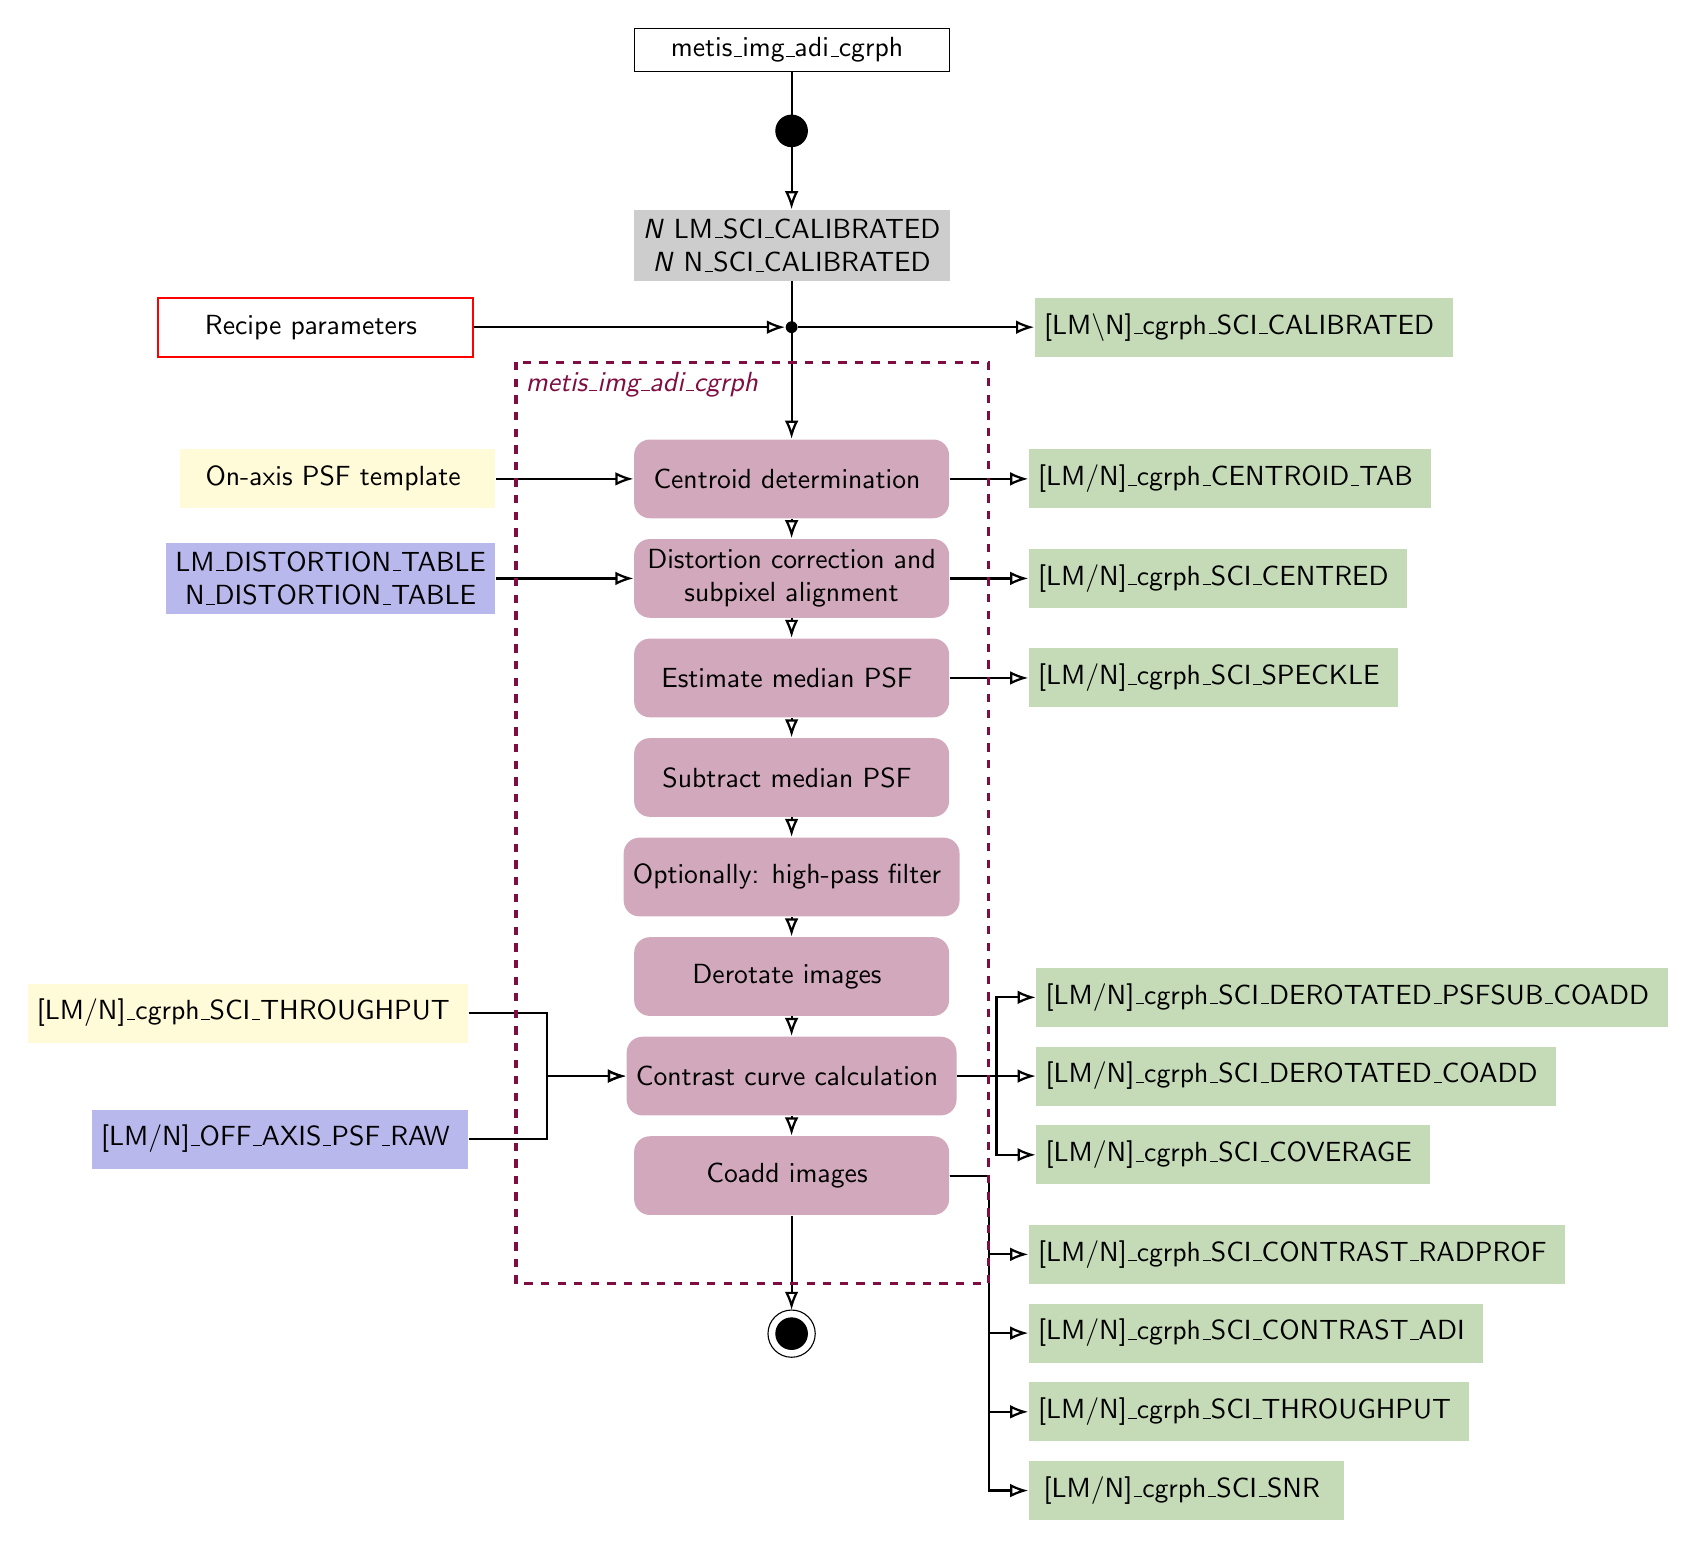
\begin{tikzpicture}
  [x=1cm,
  y=-1cm,
  align=center,
  node distance=2cm and 3cm]
  \sffamily

  %% Grid for orientation. Comment out for final figure!
% \draw[help lines, green](-8, 0) grid (8, 21);

  %%% Put workflow commands here:
  %% Main reduction workflow

  \node (template) [template]{%
   metis\_img\_adi\_cgrph
  };

  \pic (start) [below=0.75cm of template] {start};

  \node (input) [below=0.75cm of start-m, input]{%
    \textsl{N} LM\_SCI\_CALIBRATED\\
    \textsl{N} N\_SCI\_CALIBRATED
  };

  \node (step1) [below=2cm of input, redstep]{%
    Centroid determination
  };

  \node (step2)[below=0.25cm of step1, redstep]{%
    Distortion correction and\\subpixel alignment
  };

  \node (step3) [below=0.25cm of step2, redstep]{%
    Estimate median PSF
  };

  \node (step4) [below=0.25cm of step3, redstep]{%
    Subtract median PSF
  };
  \node (step4b) [below=0.25cm of step4, redstep]{%
    Optionally: high-pass filter
  };

  \node (step5) [below=0.25cm of step4b, redstep]{%
    Derotate images
  };

  \node (step6) [below=0.25cm of step5, xshift=0cm,redstep]{%
    Contrast curve calculation
  };

  \node (step7) [below=0.25cm of step6, xshift=0cm,redstep]{%
    Coadd images
  };


  \pic (stop) [below=1.5cm of step7]{stop};
  

  %% Connections
  \draw [connection_arrow] (template) -- (input);
  \draw [connection_arrow] (input) -- (step1);
  \draw [connection_arrow] (step1) -- (step2);
  \draw [connection_arrow] (step2) -- (step3);
  \draw [connection_arrow] (step3) -- (step4);
  \draw [connection_arrow] (step4) -- (step4b);
  \draw [connection_arrow] (step4b) -- (step5);
  \draw [connection_arrow] (step5) -- (step6);
  \draw [connection_arrow] (step6) -- (step7);
  \draw [connection_arrow] (step7) -- (stop-t);
  

  %% Input
  \node (connectpers) [connection] at
  ($(input)!0.35!(step1)$) {};
  %\node (persistence) [left=3.95cm of connectpers,yshift=0.8cm, external]{%
    %FLUXSTD\_CATALOG
  %};
  %\draw [connection_arrow] (persistence.east) -- ++(1., 0) -- ++(0., 0.8) -- ++(3., 0);

  % Input for detector signature removal (step1)
  %\node (bpmin) [left=2cm of step1, yshift=0.8cm, calproduct]{%
  %  BADPIX\_MAP\_IFU
  %};
  %\draw [connection_arrow] (bpmin.east) -- ++(1., 0) -- ++(0., 0.6) -- ++(1., 0);

  %\node (darkin) [left=2cm of step1, calproduct] {%
  %  MASTER\_DARK\_IFU
  %};
  %\draw [connection_arrow] (darkin) -- (step1);

  %\node (flatin) [left=2cm of step1, yshift=-0.8cm, calproduct]{%
  %  MASTER\_FLAT\_IFU
  %};
  %\draw [connection_arrow] (flatin.east) -- ++(1., 0) -- ++(0., -0.6) -- ++(1., 0);

  % Input for rectification (step3)
  %\node (wavecal) [left=2cm of step3, yshift=0.4cm, calproduct]{%
  %  IFU\_WAVECAL
  %};
  %\draw [connection_arrow] (wavecal.east) -- ++(1., 0) -- %++(0., 0.3) -- ++(1., 0);

  %\node (distortion) [left=2cm of step3, yshift=-0.4cm, calproduct]{%
  %  IFU\_DISTORT\_TAB
  %};
  %\draw [connection_arrow] (distortion.east) -- ++(1., 0) -- ++(0., -0.3) -- ++(1., 0);

  % Further input
  \node (molecparams) [right=3.cm of connectpers,yshift=0cm, sciproduct]{%
    [LM\textbackslash N]\_cgrph\_SCI\_CALIBRATED
  };
  \draw [connection_arrow] (connectpers) -- (molecparams);%-- ++(0.25, 0) -- ++(0., -0.8) -- ++(3.75, 0);
\node (molecparams2) [left=3.95cm of connectpers,yshift=0cm, params]{%
    Recipe parameters
  };
  \draw [connection_arrow] (molecparams2) -- (connectpers);

  %\node (stdcat) [left=2cm of step5, external] {%
   % FLUXSTD\_CATALOG
  %};
  %\draw [connection_arrow] (stdcat.east) -- (step5);

  %% Output
  %\node (connectreduced) [connection] at
 % ($(step5)!0.4!(stop-t)$) {};

\node (incont1) [left=2cm of step6, yshift=0.8cm,calib]{%
    [LM/N]\_cgrph\_SCI\_THROUGHPUT
  };
\draw [connection_arrow] (incont1.east) -- ++(1, 0) -- ++(0., 0.8) -- ++(1, 0);

\node (incont2) [left=2cm of step6, yshift=-0.8cm,calproduct]{%
    [LM/N]\_OFF\_AXIS\_PSF\_RAW
  };
\draw [connection_arrow] (incont2.east) -- ++(1, 0) -- ++(0., -0.8) -- ++(1, 0);

\node (outcont1) [right=1.cm of step6, yshift=1cm,sciproduct]{%
    [LM/N]\_cgrph\_SCI\_DEROTATED\_PSFSUB\_COADD
  };
\draw [connection_arrow] (step6.east) -- ++(0.5, 0) -- ++(0., -1) -- ++(0.5, 0);

\node (outcont2) [right=1.cm of step6, yshift=0cm,sciproduct]{%
    [LM/N]\_cgrph\_SCI\_DEROTATED\_COADD
  };
\draw [connection_arrow] (step6.east) -- (outcont2);

\node (outcont3) [right=1.cm of step6, yshift=-1cm,sciproduct]{%
    [LM/N]\_cgrph\_SCI\_COVERAGE
  };
\draw [connection_arrow] (step6.east) -- ++(0.5, 0) -- ++(0., 1) -- ++(0.5, 0);

\node (outcont4) [right=1.cm of step7, yshift=-1cm,sciproduct]{%
    [LM/N]\_cgrph\_SCI\_CONTRAST\_RADPROF
  };
\draw [connection_arrow] (step7.east) -- ++(0.5, 0) -- ++(0., 1) -- ++(0.5, 0);

\node (outcont5) [right=1.cm of step7, yshift=-2cm,sciproduct]{%
    [LM/N]\_cgrph\_SCI\_CONTRAST\_ADI
  };
\draw [connection_arrow] (step7.east) -- ++(0.5, 0) -- ++(0., 2) -- ++(0.5, 0);

\node (outcont6) [right=1.cm of step7, yshift=-3cm,sciproduct]{%
    [LM/N]\_cgrph\_SCI\_THROUGHPUT
  };
\draw [connection_arrow] (step7.east) -- ++(0.5, 0) -- ++(0., 3) -- ++(0.5, 0);

\node (outcont7) [right=1.cm of step7, yshift=-4cm,sciproduct]{%
    [LM/N]\_cgrph\_SCI\_SNR
  };
\draw [connection_arrow] (step7.east) -- ++(0.5, 0) -- ++(0., 4) -- ++(0.5, 0);

\node (reduced2) [right=1.cm of step1, sciproduct]{%
    [LM/N]\_cgrph\_CENTROID\_TAB
  };
  \draw [connection_arrow] (step1) -- (reduced2);
 
  \node (reduced) [right=1.cm of step2, sciproduct]{%
    [LM/N]\_cgrph\_SCI\_CENTRED
  };
  \draw [connection_arrow] (step2) -- (reduced);

  \node (reduced3) [left=1.75cm of step2, calproduct]{%
    LM\_DISTORTION\_TABLE\\
    N\_DISTORTION\_TABLE  };
  \draw [connection_arrow] (reduced3) -- (step2);
 
  \node (reduced4) [left=1.75cm of step1, calib]{%
    On-axis PSF template
  };
  \draw [connection_arrow] (reduced4) -- (step1);
 % \node (connectfluxcal) [connection] at
 % ($(step5)!0.8!(stop-t)$) {};
  \node (fluxcal) [right=1.cm of step3, sciproduct]{%
    [LM/N]\_cgrph\_SCI\_SPECKLE
  };
  \draw [connection_arrow] (step3) -- (fluxcal);

  %% Frame around recipe
  \draw [frame] ($(input)!0.5!(step1) - (3.5,0)$)
  rectangle ($(step7)!0.75!(stop-t) + (2.5,0)$);
  \node [framecolor, anchor=north west] at
  ($(input)!0.5!(step1) - (3.5, 0)$) {%
    \textsl{metis\_img\_adi\_cgrph}};

\end{tikzpicture}

% ADDING NEW DEFINITIONS -------------------------------------------- start
\definecolor{listingbg}{gray}{0.95}
\definecolor{darkgreen}{rgb}{0.0, 0.7, 0.0}
\definecolor{darkblue} {rgb}{0.0, 0.0, 0.7}
\definecolor{cyan} {rgb}{0.0, 0.4, 0.4}
\definecolor{darkred}  {rgb}{0.7, 0.0, 0.0}
\definecolor{darkorange}{rgb}{1.0, 0.49, 0.0}
\definecolor{violet}{rgb}{255, 0, 255}
\definecolor{turq}{rgb}{0.0, 0.7, 0.8}
\definecolor{fits}{rgb}{0.4, 0.1, 1}


\makeatletter
\lstdefinestyle{RAWstyle}{%
  basicstyle=\ttfamily\color{fits}%
  \lst@ifdisplaystyle\scriptsize\fi}

\lstdefinestyle{PARstyle}{%
  basicstyle=\ttfamily\color{cyan}%
  \lst@ifdisplaystyle\scriptsize\fi}

\lstdefinestyle{DRLstyle}{%
  basicstyle=\ttfamily\color{violet}%
  \lst@ifdisplaystyle\scriptsize\fi}

\lstdefinestyle{RECstyle}{%
  basicstyle=\ttfamily\color{darkgreen}%
  \lst@ifdisplaystyle\scriptsize\fi}

%% Write QC parameters like this: \QC{QC_SOMETHING_OR_OTHER}
\lstdefinestyle{QCstyle}{%
  basicstyle=\ttfamily\color{darkblue}%
  \lst@ifdisplaystyle\scriptsize\fi}

%% Write templates like this: \TPL{DARK_LM}
\lstdefinestyle{TPLstyle}{%
  basicstyle=\ttfamily\color{darkred}%
  \lst@ifdisplaystyle\scriptsize\fi}

%% Write products like this: \hyperref[dataitem:some_thing]{\PROD{SOME_THING}}
\lstdefinestyle{PRODstyle}{%
  basicstyle=\ttfamily\color{darkorange}%
  \lst@ifdisplaystyle\scriptsize\fi}

%% external calib files
\lstdefinestyle{EXTCALIBstyle}{%
  basicstyle=\ttfamily\color{Turquoise}%
  \lst@ifdisplaystyle\scriptsize\fi}

% static calib files
\lstdefinestyle{STATCALIBstyle}{%
  basicstyle=\ttfamily\color{teal}%
  \lst@ifdisplaystyle\scriptsize\fi}
\makeatother

  \caption[Recipe: \REC*{metis_img_adi_cgrph}]{\REC{metis_img_adi_cgrph} -- DET ADI post processing for RAVC/CVC coronagraph.
    }
  \label{fig:metis_det_adi_ravc}
\end{figure}
\restoregeometry

%------------------------------------------------------------------------------------------------------------------
\subsubsection{\REC*{metis_lm_adi_app}: IMG\_LM APP ADI post processing}
\label{sssec:adi_img_app}


The following recipe is applicable for ADI post processing for the LM
band, in combination with the APP coronagraph. It is very
similar to the recipe for RAVC/CVC coronagraphs, with the
addition of steps for merging together the two half PSFs, and of
applying an angular wedge mask before the derotation and stacking, and
contrast curve calculations steps. An input set of observations
consists of a time sequence of ADI images in LM band, which have
already undergone basic calibration.

For each image, the centroid of the central source is determined for
all three PSFs and distortion corrections are performed. The PSFs are
aligned at a sub-pixel scale and extracted; the extracted
coronagraphic PSFs are merged to produce a complete PSF and the third
PSF is used to form a cube of calibrated leakage PSFs.  The
mean/median/sigmaclipped PSF is estimated and subtracted from each
frame of the merged coronagraphic PSF. Each image is then derotated to
place the off-axis source at the same on-sky angle and coadded to
produce the final stacked science image. In addition, the images prior
to PSF subtraction are derotated and combined to produce a second
final stacked image.

In addition to the final images, the stack of derotated, PSF
subtracted images are used to calculate the raw and post-ADI contrast
curves as well as the ADI throughput curve and coverage map containing
the effective number of included frames.





\begin{recipedef}\label{rec:metis_lm_adi_app}
  Name:                & \REC{metis_lm_adi_app}                                        \\
  Purpose:             & Classical ADI post processing for APP coronagraph      \\
  Requirements:        & \REQ{METIS-5989}                                               \\
  Templates:           & None                               \\
  Type:                & Science                                                    \\
  Input data:          & \PROD{LM_SCI_CALIBRATED}                            \\
                       & \PROD{LM_DISTORTION_TABLE} \\
                       & \RAW{LM_OFF_AXIS_PSF_RAW}                                                  \\
   Matched keywords:   & \FITS{DRS.MASK} \\
   Parameters:         & combination method (median, mean, sigclip, \dots) \\
                       & parameters for combination method         \\
                       & resampling method \\
                       & parameters for resampling method \\
                       & start and end limit to contrast curve (in $\lambda/D$) \\
                       & frame exclusion thresholds dependent on AO parameters and centroid offset \\
% HB 20230627: There is no APP in the N-band right?
%   Algorithm:           & call \DRL{lm_adi_app_centroid} or  \DRL{n_adi_app_centroid} to determine the centroids of the central PSFs \\
%                        & call \DRL{adi_regrid} to apply distortion map and regrid images based on position of central PSFs \\
%                        & call \DRL{lm_merge_app_adi_psf} of  \DRL{n_merge_app_adi_psf} to merge the coronagraphic PSFs \\
%                        & call \DRL{lm_adi_app_psf} or \DRL{n_adi_app_psf} to determine the median PSF \\
  Algorithm:           & call \DRL{lm_adi_app_centroid} to determine the centroids of the central PSFs \\
                       & call \DRL{adi_regrid} to apply distortion map and regrid images based on position of central PSFs \\
                       & call \DRL{lm_merge_app_adi_psf} to merge the coronagraphic PSFs \\
                       & call \DRL{lm_adi_app_psf} to determine the median PSF \\
                       & Subtract median PSF from all frames  (\CODE{hdrl_imagelist_sub_image})\\
                       & call \DRL{adi_derotate} to derotate both PSF subtracted and unsubtracted images \\
                       & coadd derotated images with image mask   (\CODE{hdrl_imagelist_collapse})\\
                       & call \DRL{lm_adi_app_contrast} for raw and post processed images \\
  Output data:       & \PROD{LM_APP_SCI_CALIBRATED}\\
                     & \PROD{LM_APP_SCI_CENTRED}\\
                     & \PROD{LM_APP_CENTROID_TAB}\\
                     & \PROD{LM_APP_SCI_SPECKLE}\\
                     & \PROD{LM_APP_SCI_DEROTATED_PSFSUB}\\
                     & \PROD{LM_APP_SCI_DEROTATED}\\
                     & \PROD{LM_APP_SCI_CONTRAST_RADPROF}\\
                     & \PROD{LM_APP_SCI_CONTRAST_ADI}\\
                     & \PROD{LM_APP_SCI_THROUGHPUT}\\
                     & \PROD{LM_APP_SCI_COVERAGE}\\
                     & \PROD{LM_APP_SCI_SNR}\\
                     & \PROD{LM_APP_PSF_MEDIAN}\\
Expected accuracies: & n/a                                                           \\
QC1 parameters:  & \QC{QC det APP SCI NEXPOSURES}\\
                 & \QC{QC det APP SCI FWHM nn}\\
                 & \QC{QC det APP SCI SNR MEAN}\\
                 & \QC{QC det APP SCI SNR PEAK}\\
                 & \QC{QC det APP SCI CONTRAST RAW LAMD}\\
                 & \QC{QC det APP SCI CONTRAST ADI LAMD}\\
  hdrl functions:      & \CODE{hdrl_imagelist_collapse}     \\
                       & \CODE{hdrl_imagelist_sub_image}        \\
                       & \CODE{hdrl_catalogue_compute}       \\
                       & \CODE{hdrl_resample_compute}       \\
\end{recipedef}

\newgeometry{bottom=0.1cm, right=0.1cm, left=0.1cm}
\begin{figure}[hb]
  \centering
  \def \globalscale {0.400000}
  \fontsize{10}{12}\selectfont
  

% ADDING NEW DEFINITIONS -------------------------------------------- start
\definecolor{listingbg}{gray}{0.95}
\definecolor{darkgreen}{rgb}{0.0, 0.7, 0.0}
\definecolor{darkblue} {rgb}{0.0, 0.0, 0.7}
\definecolor{cyan} {rgb}{0.0, 0.4, 0.4}
\definecolor{darkred}  {rgb}{0.7, 0.0, 0.0}
\definecolor{darkorange}{rgb}{1.0, 0.49, 0.0}
\definecolor{violett}{rgb}{255, 0, 255}
\definecolor{turq}{rgb}{0.0, 0.7, 0.8}
\definecolor{fits}{rgb}{0.4, 0.1, 1}


\makeatletter
\lstdefinestyle{RAWstyle}{%
  basicstyle=\ttfamily\color{black}%
  \lst@ifdisplaystyle\scriptsize\fi}

\lstdefinestyle{PARstyle}{%
  basicstyle=\ttfamily\color{black}%
  \lst@ifdisplaystyle\scriptsize\fi}

\lstdefinestyle{DRLstyle}{%
  basicstyle=\ttfamily\color{black}%
  \lst@ifdisplaystyle\scriptsize\fi}

\lstdefinestyle{RECstyle}{%
  basicstyle=\ttfamily\color{black}%
  \lst@ifdisplaystyle\scriptsize\fi}

\lstdefinestyle{QCstyle}{%
  basicstyle=\ttfamily\color{black}%
  \lst@ifdisplaystyle\scriptsize\fi}

\lstdefinestyle{TPLstyle}{%
  basicstyle=\ttfamily\color{black}%
  \lst@ifdisplaystyle\scriptsize\fi}

\lstdefinestyle{PRODstyle}{%
  basicstyle=\ttfamily\color{black}%
  \lst@ifdisplaystyle\scriptsize\fi}

\lstdefinestyle{EXTCALIBstyle}{%
  basicstyle=\ttfamily\color{black}%
  \lst@ifdisplaystyle\scriptsize\fi}

\lstdefinestyle{STATCALIBstyle}{%
  basicstyle=\ttfamily\color{black}%
  \lst@ifdisplaystyle\scriptsize\fi}
\makeatother

%%% This file contains definitions of shapes and nodes used
%%% for a recipe workflow
%%% Author       : Oliver Czoske
%%% Created      : 2021-03-03
%%% Last Changed : 2021-03-03
%%% Changes:
%%%

\usetikzlibrary{
  shapes.misc,
  positioning,
  calc,
  arrows.meta}

%% All connecting lines have an arrow
\tikzset{
  connection_arrow/.style={->, >=Latex[open], thick}
}

%% Start and stop buttons (black disks, stop with ring)
%% These are pics, use as
%%         \pic (name) [above of=..] {picname};
\tikzset{
  start/.pic = {
    \node (-m) at (0, 0){};
    \filldraw [fill=black] (0, 0) circle (0.2);
  }
}

\tikzset{
  stop/.pic = {
    \node (-m) at (0, 0){};
    \node (-t) at (0, -0.3){};
    \filldraw [fill=black] (0, 0) circle(0.2);
    \draw[black] (0, 0) circle (0.3);
  }
}


%%%% Various boxes and their colours
%%%% These are nodes, use as
%%%% \node (name) [type, location]  {text};

\definecolor{stepcolor}{RGB}{210,169,188}
\definecolor{rawcolor}{RGB}{205,205,205}
\definecolor{externalcolor}{RGB}{183,255,255}
\definecolor{calibcolor}{RGB}{255,250,216}
\definecolor{calproductcolor}{RGB}{185,184,237}
\definecolor{qcproductcolor}{RGB}{255,201,165}
\definecolor{sciproductcolor}{RGB}{197,219,183}
\definecolor{framecolor}{RGB}{127,13,65}

\tikzset{
  %% template : the template(s) that trigger(s) the recipe
  template/.style={
    rectangle,
    draw=black,
    minimum width=4.0cm,
    minimum height=0.5cm,
    align=center
  },
  %% input : the input files
  input/.style={
    rectangle,
    fill=rawcolor,
    minimum width=4.0cm,
    minimum height=0.75cm,
%     text width=3cm,
    align=center
  },
  %% calib : calibration input
  calib/.style={
    rectangle,
    fill=calibcolor,
    minimum width=4.0cm,
    minimum height=0.75cm,
%     text width=3cm,
    align=center
  },
  %% external : external input
  external/.style={
    rectangle,
    fill=externalcolor,
    minimum width=4.0cm,
    minimum height=0.75cm,
%     text width=3.5cm,
    align=center
  },
  %% params : parameters
  params/.style={
    rectangle,
    draw=red,
    thick,
    minimum width=4.0cm,
    minimum height=0.75cm,
%     text width=3cm,
    align=center
  },
  %% redstep : a reduction step
  %%      ("step" is predefined and can't be used)
  redstep/.style={
    rectangle,
    rounded corners=0.2cm,
    fill=stepcolor,   %%% define colour!
    minimum width=4.0cm,
    minimum height=1cm,
%     text width=3cm,
    align=center
  },
  %% connection : connection to input or output
  connection/.style={
    circle,
    fill=black,
    minimum size=0.15cm,
    inner sep=0pt
  },
  %% sciproduct : a science product
  sciproduct/.style={
    rectangle,
    fill=sciproductcolor,
    minimum width=4.0cm,
    minimum height=0.75cm,
%     text width=3.5cm,
    align=center
  },
  %% calproduct : a calibration product
  calproduct/.style={
    rectangle,
    fill=calproductcolor,
    minimum width=4.0cm,
    minimum height=0.75cm,
%     text width=3.5cm,
    align=center
  },
  %% frame : frame around the recipe
  %% This is a path, use as
  %%    \draw [frame] (upper left) rectangle (lower right);
  frame/.style={framecolor, very thick, dashed}
}

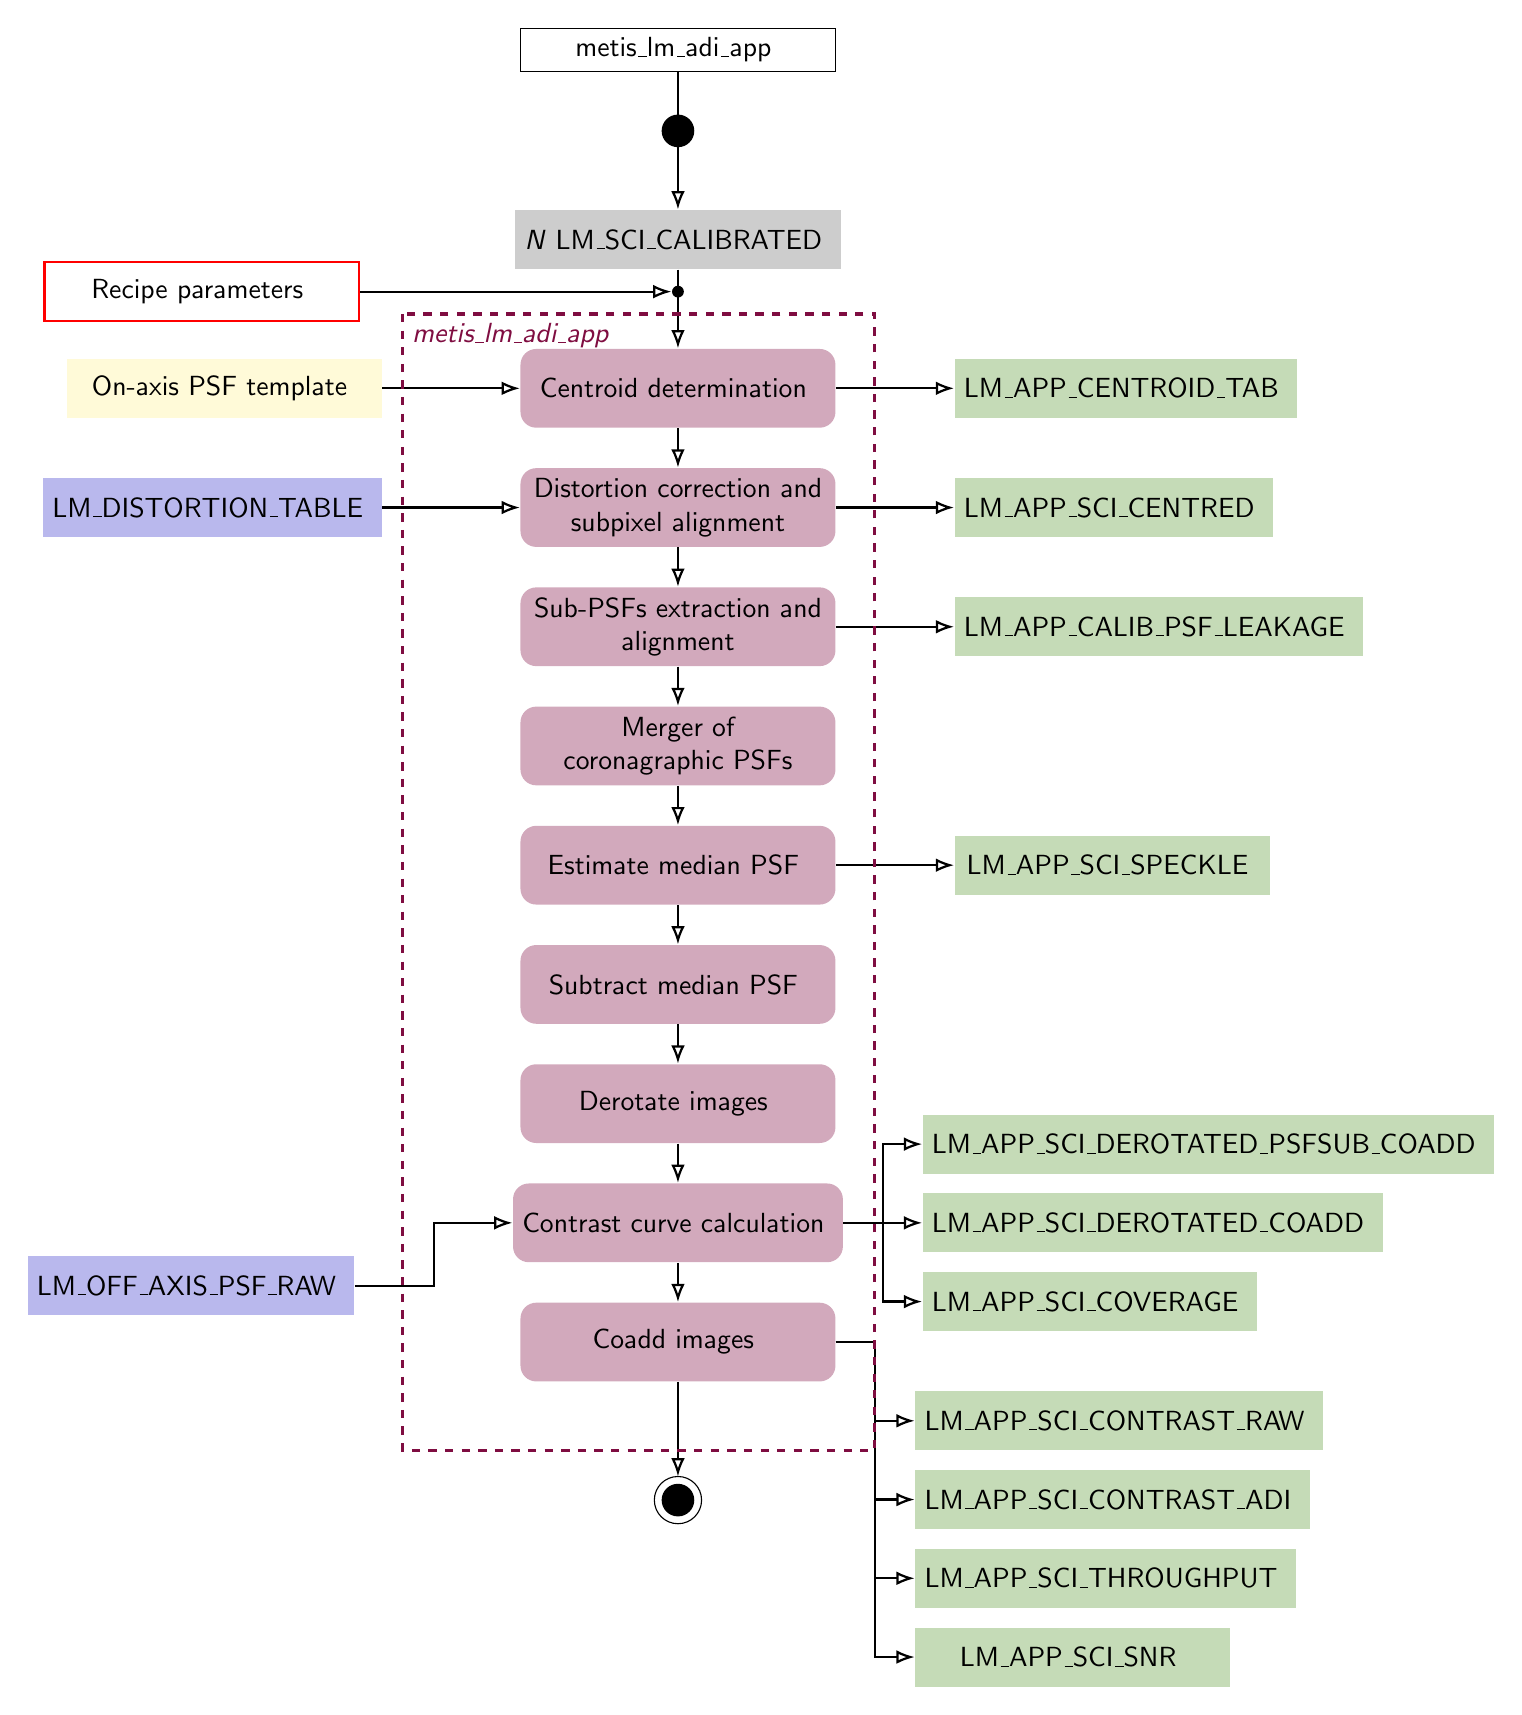
\begin{tikzpicture}
  [x=1cm,
  y=-1cm,
  align=center,
  node distance=2cm and 3cm]
  \sffamily

  %% Grid for orientation. Comment out for final figure!
 %\draw[help lines, green](-8, 0) grid (8, 21);

  %%% Put workflow commands here:
  %% Main reduction workflow

  \node (template) [template]{%
   metis\_lm\_adi\_app
  };

  \pic (start) [below=0.75cm of template] {start};

  \node (input) [below=0.75cm of start-m, input]{%
    \textsl{N} LM\_SCI\_CALIBRATED
  };

  \node (step1) [below=1cm of input, redstep]{%
    Centroid determination
  };

  \node (step2)[below=0.5cm of step1, redstep]{%
    Distortion correction and\\subpixel alignment
  };

\node (step2a) [below=0.5cm of step2, redstep]{%
    Sub-PSFs extraction and\\ alignment
  };

  \node (step2b) [below=0.5cm of step2a, redstep]{%
    Merger of \\ coronagraphic PSFs
  };


  \node (step3) [below=0.5cm of step2b, redstep]{%
    Estimate median PSF
  };

  \node (step4) [below=0.5cm of step3, redstep]{%
    Subtract median PSF
  };

  \node (step5) [below=0.5cm of step4, redstep]{%
    Derotate images
  };

  \node (step6) [below=0.5cm of step5, xshift=0cm,redstep]{%
    Contrast curve calculation
  };

  \node (step7) [below=0.5cm of step6, xshift=0cm,redstep]{%
    Coadd images
  };


  \pic (stop) [below=1.5cm of step7]{stop};
  

  %% Connections
  \draw [connection_arrow] (template) -- (input);
  \draw [connection_arrow] (input) -- (step1);
  \draw [connection_arrow] (step1) -- (step2);
  \draw [connection_arrow] (step2) -- (step2a);
  \draw [connection_arrow] (step2a) -- (step2b);
  \draw [connection_arrow] (step2b) -- (step3);
  \draw [connection_arrow] (step3) -- (step4);
  \draw [connection_arrow] (step4) -- (step5);
  \draw [connection_arrow] (step5) -- (step6);
  \draw [connection_arrow] (step6) -- (step7);
  \draw [connection_arrow] (step7) -- (stop-t);
  

  %% Input
  \node (connectpers) [connection] at
  ($(input)!0.35!(step1)$) {};
  %\node (persistence) [left=3.95cm of connectpers,yshift=0.8cm, external]{%
    %FLUXSTD\_CATALOG
  %};
  %\draw [connection_arrow] (persistence.east) -- ++(1., 0) -- ++(0., 0.8) -- ++(3., 0);

  % Input for detector signature removal (step1)
  %\node (bpmin) [left=2cm of step1, yshift=0.8cm, calproduct]{%
  %  BADPIX\_MAP\_IFU
  %};
  %\draw [connection_arrow] (bpmin.east) -- ++(1., 0) -- ++(0., 0.6) -- ++(1., 0);

  %\node (darkin) [left=2cm of step1, calproduct] {%
  %  MASTER\_DARK\_IFU
  %};
  %\draw [connection_arrow] (darkin) -- (step1);

  %\node (flatin) [left=2cm of step1, yshift=-0.8cm, calproduct]{%
  %  MASTER\_FLAT\_IFU
  %};
  %\draw [connection_arrow] (flatin.east) -- ++(1., 0) -- ++(0., -0.6) -- ++(1., 0);

  % Input for rectification (step3)
  %\node (wavecal) [left=2cm of step3, yshift=0.4cm, calproduct]{%
  %  IFU\_WAVECAL
  %};
  %\draw [connection_arrow] (wavecal.east) -- ++(1., 0) -- %++(0., 0.3) -- ++(1., 0);

  %\node (distortion) [left=2cm of step3, yshift=-0.4cm, calproduct]{%
  %  IFU\_DISTORT\_TAB
  %};
  %\draw [connection_arrow] (distortion.east) -- ++(1., 0) -- ++(0., -0.3) -- ++(1., 0);

  % Further input
  \node (molecparams) [left=3.95cm of connectpers,yshift=0cm, params]{%
    Recipe parameters
  };
  \draw [connection_arrow] (molecparams.east) -- (connectpers);%-- ++(0.25, 0) -- ++(0., -0.8) -- ++(3.75, 0);

  %\node (stdcat) [left=2cm of step5, external] {%
   % FLUXSTD\_CATALOG
  %};
  %\draw [connection_arrow] (stdcat.east) -- (step5);

  %% Output
  %\node (connectreduced) [connection] at
 % ($(step5)!0.4!(stop-t)$) {};

 

%\node (incont1) [left=2cm of step6, yshift=0.8cm,calib]{%
 %   Coronagraphic throughput\\map/profile
 % };
%\draw [connection_arrow] (incont1.east) -- ++(1, 0) -- ++(0., 0.8) -- ++(1, 0);

\node (incont2) [left=2cm of step6, yshift=-0.8cm,calproduct]{%
    LM\_OFF\_AXIS\_PSF\_RAW
  };
\draw [connection_arrow] (incont2.east) -- ++(1, 0) -- ++(0., -0.8) -- ++(1, 0);

\node (outcont1) [right=1.cm of step6, yshift=1cm,sciproduct]{%
    LM\_APP\_SCI\_DEROTATED\_PSFSUB\_COADD
  };
\draw [connection_arrow] (step6.east) -- ++(0.5, 0) -- ++(0., -1) -- ++(0.5, 0);

\node (outcont2) [right=1.cm of step6, yshift=0cm,sciproduct]{%
    LM\_APP\_SCI\_DEROTATED\_COADD
  };
\draw [connection_arrow] (step6.east) -- (outcont2);

\node (outcont3) [right=1.cm of step6, yshift=-1cm,sciproduct]{%
    LM\_APP\_SCI\_COVERAGE
  };
\draw [connection_arrow] (step6.east) -- ++(0.5, 0) -- ++(0., 1) -- ++(0.5, 0);

\node (outcont4) [right=1.cm of step7, yshift=-1cm,sciproduct]{%
    LM\_APP\_SCI\_CONTRAST\_RAW
  };
\draw [connection_arrow] (step7.east) -- ++(0.5, 0) -- ++(0., 1) -- ++(0.5, 0);

\node (outcont5) [right=1.cm of step7, yshift=-2cm,sciproduct]{%
    LM\_APP\_SCI\_CONTRAST\_ADI
  };
\draw [connection_arrow] (step7.east) -- ++(0.5, 0) -- ++(0., 2) -- ++(0.5, 0);

\node (outcont6) [right=1.cm of step7, yshift=-3cm,sciproduct]{%
    LM\_APP\_SCI\_THROUGHPUT
  };
\draw [connection_arrow] (step7.east) -- ++(0.5, 0) -- ++(0., 3) -- ++(0.5, 0);

\node (outcont7) [right=1.cm of step7, yshift=-4cm,sciproduct]{%
    LM\_APP\_SCI\_SNR
  };
\draw [connection_arrow] (step7.east) -- ++(0.5, 0) -- ++(0., 4) -- ++(0.5, 0);

\node (reduced2) [right=1.5cm of step1, sciproduct]{%
    LM\_APP\_CENTROID\_TAB
  };
  \draw [connection_arrow] (step1) -- (reduced2);
 
  \node (reduced) [right=1.5cm of step2, sciproduct]{%
    LM\_APP\_SCI\_CENTRED
  };
  \draw [connection_arrow] (step2) -- (reduced);

  \node (reduced3) [left=1.75cm of step2, calproduct]{%
    LM\_DISTORTION\_TABLE
  };
  \draw [connection_arrow] (reduced3) -- (step2);

  \node (reduced4) [left=1.75cm of step1, calib]{%
    On-axis PSF template
  };
  \draw [connection_arrow] (reduced4) -- (step1);

 % \node (connectfluxcal) [connection] at
 % ($(step5)!0.8!(stop-t)$) {};
  \node (fluxcal) [right=1.5cm of step3, sciproduct]{%
    LM\_APP\_SCI\_SPECKLE
  };
  \draw [connection_arrow] (step3) -- (fluxcal);

\node (fluxcal2) [right=1.5cm of step2a, sciproduct]{%
    LM\_APP\_CALIB\_PSF\_LEAKAGE
  };
  \draw [connection_arrow] (step2a) -- (fluxcal2);


  %% Frame around recipe
  \draw [frame] ($(input)!0.5!(step1) - (3.5,0)$)
  rectangle ($(step7)!0.75!(stop-t) + (2.5,0)$);
  \node [framecolor, anchor=north west] at
  ($(input)!0.5!(step1) - (3.5, 0)$) {%
    \textsl{metis\_lm\_adi\_app}};

\end{tikzpicture}

% ADDING NEW DEFINITIONS -------------------------------------------- start
\definecolor{listingbg}{gray}{0.95}
\definecolor{darkgreen}{rgb}{0.0, 0.7, 0.0}
\definecolor{darkblue} {rgb}{0.0, 0.0, 0.7}
\definecolor{cyan} {rgb}{0.0, 0.4, 0.4}
\definecolor{darkred}  {rgb}{0.7, 0.0, 0.0}
\definecolor{darkorange}{rgb}{1.0, 0.49, 0.0}
\definecolor{violet}{rgb}{255, 0, 255}
\definecolor{turq}{rgb}{0.0, 0.7, 0.8}
\definecolor{fits}{rgb}{0.4, 0.1, 1}


\makeatletter
\lstdefinestyle{RAWstyle}{%
  basicstyle=\ttfamily\color{fits}%
  \lst@ifdisplaystyle\scriptsize\fi}

\lstdefinestyle{PARstyle}{%
  basicstyle=\ttfamily\color{cyan}%
  \lst@ifdisplaystyle\scriptsize\fi}

\lstdefinestyle{DRLstyle}{%
  basicstyle=\ttfamily\color{violet}%
  \lst@ifdisplaystyle\scriptsize\fi}

\lstdefinestyle{RECstyle}{%
  basicstyle=\ttfamily\color{darkgreen}%
  \lst@ifdisplaystyle\scriptsize\fi}

%% Write QC parameters like this: \QC{QC_SOMETHING_OR_OTHER}
\lstdefinestyle{QCstyle}{%
  basicstyle=\ttfamily\color{darkblue}%
  \lst@ifdisplaystyle\scriptsize\fi}

%% Write templates like this: \TPL{DARK_LM}
\lstdefinestyle{TPLstyle}{%
  basicstyle=\ttfamily\color{darkred}%
  \lst@ifdisplaystyle\scriptsize\fi}

%% Write products like this: \hyperref[dataitem:some_thing]{\PROD{SOME_THING}}
\lstdefinestyle{PRODstyle}{%
  basicstyle=\ttfamily\color{darkorange}%
  \lst@ifdisplaystyle\scriptsize\fi}

%% external calib files
\lstdefinestyle{EXTCALIBstyle}{%
  basicstyle=\ttfamily\color{Turquoise}%
  \lst@ifdisplaystyle\scriptsize\fi}

% static calib files
\lstdefinestyle{STATCALIBstyle}{%
  basicstyle=\ttfamily\color{teal}%
  \lst@ifdisplaystyle\scriptsize\fi}
\makeatother


  \caption[Recipe: \REC*{metis_lm_adi_app}]{\REC*{metis_lm_adi_app} -- ADI post processing for APP coronagraph.
    }
  \label{fig:metis_lm_adi_app}
\end{figure}
\restoregeometry

%------------------------------------------------------------------------------------------------------------------
\subsubsection{\REC*{metis_ifu_adi_cgrph}: IFU ADI post processing}
\label{sssec:adi_ifu}


The following recipe is applicable for ADI post processing for the IFU
data cubes and the RAVC/CVC and APP coronagraphs. As only a single
target can be targeted in the limited field of view the methods
overlap between coronagraphs.  For the IFU observations, the input is
a set of reduced 3D (spectral and spatial) data cubes on a rectified
grid. Note that the reduction steps after the square pixel reconstruction
are essentially identical to the non-IFU case, except for an added dimension
to loop over. 

For each wavelength slice in each cube the centroid is determined by a
QACITS-like algorithm in the case of the focal plane coronagraphs
(RAVC/CVC) or through 2D cross-correlation with a template PSF for the
APP coronagraph. This centroid information is stored in a table
together with timestamps, parallactic angle and bad frame flags (based
on AO loop status, AO performance, atmospheric parameters and centroid
offset).  As the ADI step requires square pixels following previous
work on combining ADI techniques with IFUs (such as SPHERE/IFS,
SINFONI), the rectangular spatial grid is interpolated or nearest
neighbor filled to produce a square pixel image.  It is acknowledged
that one spatial dimension is undersampled which may lead to reduced
performance compared to a Nyquist-sampled PSF.  The
mean/median/sigmaclipped PSF (in time) is estimated for each
wavelength and subtracted from each image in the cube.  After
derotation the cubes are combined in time to give a coadded cube. For
the APP a wedge shape is used. The limited field of view of the IFU
means that only one APP dark hole can be centered on the IFU. The derotated cubes
are also used to generate post ADI contrast curves and contrast curves
with input from the radial coronagraph throughput profile and off-axis
PSFs. In addition coverage maps are produced.

% TODO: Perhaps integrate this comment by GO:
%So if you inject a fake planet with a known brightness and retrieve it at a 5 sigma level after ADI processing, the brightness of that source with respect to the unobscured stellar brightness defines the post-ADI contrast at a certain location. You can repeat this azimuthally and radially to get a complete map of the contrast around the star which is converted into a radial contrast curve.

%While not part of the PIP specs, the current generation of VIP\_HCI
%ADI reduction algorithms supports the more detailed Marois et al. 2006
%ADI routine, PCA-based routines, as well as ADI+mSDI processing to
%improve the speckle PSF estimation with the additional wavelength
%information.



\begin{recipedef}
  Name:                & \REC{metis_ifu_adi_cgrph}\label{rec:metis_ifu_adi_cgrph}                                        \\
  Purpose:             & Classical ADI post processing for APP/CVC/RAVC coronagraphs with IFU      \\
  Requirements:        & \REQ{METIS-5989}                                               \\
  Templates:           & None                               \\
  Type:                & Science                                                    \\
  Input data:          & \PROD{IFU_SCI_CUBE_CALIBRATED}                            \\
                       & \PROD{IFU_DISTORTION_TABLE}\\
%                        & Coronagraphic throughput map and profile                                                  \\
                       & \PROD{IFU_cgrph_SCI_THROUGHPUT} \\
                       & \RAW{IFU_OFF_AXIS_PSF_RAW} \\
   Matched keywords:   & \FITS{DRS.MASK} \\
  Parameters:          & combination method (median, mean, sigclip, \dots)\\
                       & parameters for combination method        \\
                       & resampling method \\
                       & parameters for resampling method \\
                       & start and end limit to contrast curve (in $\lambda/D$) \\
                       & frame exclusion thresholds dependent on AO parameters and centroid offset \\
  Algorithm:           & call \DRL*{det_adi_cgrph_centroid} to determine the location of the central PSFs \\
                       & call \DRL{ifu_adi_regrid} to perform distortion correction, square pixel reconstruction and sub-pixel alignment   \\
                       & call \DRL*{det_adi_cgrph_psf} to determine the median PSF \\
                       & Subtract median PSF from all frames  (\CODE{hdrl_imagelist_sub_image})\\
                       & call \DRL{adi_derotate} to derotate both PSF subtracted and unsubtracted images \\
                       & coadd derotated images   (\CODE{hdrl_imagelist_collapse})\\
                       & call \CODE{det_adi_cgrph_contrast} for raw and post processed images \\
  Output data:       & \PROD{IFU_cgrph_SCI_CALIBRATED}\\
                     & \PROD{IFU_cgrph_SCI_CENTRED}\\
                     & \PROD{IFU_cgrph_CENTROID_TAB}\\
                     & \PROD{IFU_cgrph_SCI_SPECKLE}\\
                     & \PROD{IFU_cgrph_SCI_DEROTATED_PSFSUB}\\
                     & \PROD{IFU_cgrph_SCI_DEROTATED}\\
                     & \PROD{IFU_cgrph_SCI_CONTRAST_RADPROF}\\
                     & \PROD{IFU_cgrph_SCI_CONTRAST_ADI}\\
                     & \PROD{IFU_cgrph_SCI_THROUGHPUT}\\
                     & \PROD{IFU_cgrph_SCI_SNR}\\
                     & \PROD{IFU_cgrph_SCI_COVERAGE}                           \\

  Expected accuracies: & n/a                                                           \\
  QC1 parameters: & \QC{QC IFU cgrph SCI NEXPOSURES}\\
                  & \QC{QC IFU cgrph SCI FWHM nn}\\
                  & \QC{QC IFU cgrph SCI SNR MEAN}\\
                  & \QC{QC IFU cgrph SCI SNR PEAK}\\
                  & \QC{QC IFU cgrph SCI CONTRAST RAW LAMD}\\
                  & \QC{QC IFU cgrph SCI CONTRAST ADI LAMD}\\
  hdrl functions:      & \CODE{hdrl_imagelist_collapse}     \\
                       & \CODE{hdrl_imagelist_sub_image}        \\
                       & \CODE{hdrl_catalogue_compute}       \\
                       & \CODE{hdrl_resample_compute}       \\
\end{recipedef}

\newgeometry{bottom=0.5cm, right=0.1cm, left=0.1cm}
\begin{figure}[hb]
  \centering
  \def \globalscale {0.400000}
  \fontsize{10}{12}\selectfont
  

% ADDING NEW DEFINITIONS -------------------------------------------- start
\definecolor{listingbg}{gray}{0.95}
\definecolor{darkgreen}{rgb}{0.0, 0.7, 0.0}
\definecolor{darkblue} {rgb}{0.0, 0.0, 0.7}
\definecolor{cyan} {rgb}{0.0, 0.4, 0.4}
\definecolor{darkred}  {rgb}{0.7, 0.0, 0.0}
\definecolor{darkorange}{rgb}{1.0, 0.49, 0.0}
\definecolor{violett}{rgb}{255, 0, 255}
\definecolor{turq}{rgb}{0.0, 0.7, 0.8}
\definecolor{fits}{rgb}{0.4, 0.1, 1}


\makeatletter
\lstdefinestyle{RAWstyle}{%
  basicstyle=\ttfamily\color{black}%
  \lst@ifdisplaystyle\scriptsize\fi}

\lstdefinestyle{PARstyle}{%
  basicstyle=\ttfamily\color{black}%
  \lst@ifdisplaystyle\scriptsize\fi}

\lstdefinestyle{DRLstyle}{%
  basicstyle=\ttfamily\color{black}%
  \lst@ifdisplaystyle\scriptsize\fi}

\lstdefinestyle{RECstyle}{%
  basicstyle=\ttfamily\color{black}%
  \lst@ifdisplaystyle\scriptsize\fi}

\lstdefinestyle{QCstyle}{%
  basicstyle=\ttfamily\color{black}%
  \lst@ifdisplaystyle\scriptsize\fi}

\lstdefinestyle{TPLstyle}{%
  basicstyle=\ttfamily\color{black}%
  \lst@ifdisplaystyle\scriptsize\fi}

\lstdefinestyle{PRODstyle}{%
  basicstyle=\ttfamily\color{black}%
  \lst@ifdisplaystyle\scriptsize\fi}

\lstdefinestyle{EXTCALIBstyle}{%
  basicstyle=\ttfamily\color{black}%
  \lst@ifdisplaystyle\scriptsize\fi}

\lstdefinestyle{STATCALIBstyle}{%
  basicstyle=\ttfamily\color{black}%
  \lst@ifdisplaystyle\scriptsize\fi}
\makeatother

%%% This file contains definitions of shapes and nodes used
%%% for a recipe workflow
%%% Author       : Oliver Czoske
%%% Created      : 2021-03-03
%%% Last Changed : 2021-03-03
%%% Changes:
%%%

\usetikzlibrary{
  shapes.misc,
  positioning,
  calc,
  arrows.meta}

%% All connecting lines have an arrow
\tikzset{
  connection_arrow/.style={->, >=Latex[open], thick}
}

%% Start and stop buttons (black disks, stop with ring)
%% These are pics, use as
%%         \pic (name) [above of=..] {picname};
\tikzset{
  start/.pic = {
    \node (-m) at (0, 0){};
    \filldraw [fill=black] (0, 0) circle (0.2);
  }
}

\tikzset{
  stop/.pic = {
    \node (-m) at (0, 0){};
    \node (-t) at (0, -0.3){};
    \filldraw [fill=black] (0, 0) circle(0.2);
    \draw[black] (0, 0) circle (0.3);
  }
}


%%%% Various boxes and their colours
%%%% These are nodes, use as
%%%% \node (name) [type, location]  {text};

\definecolor{stepcolor}{RGB}{210,169,188}
\definecolor{rawcolor}{RGB}{205,205,205}
\definecolor{externalcolor}{RGB}{183,255,255}
\definecolor{calibcolor}{RGB}{255,250,216}
\definecolor{calproductcolor}{RGB}{185,184,237}
\definecolor{qcproductcolor}{RGB}{255,201,165}
\definecolor{sciproductcolor}{RGB}{197,219,183}
\definecolor{framecolor}{RGB}{127,13,65}

\tikzset{
  %% template : the template(s) that trigger(s) the recipe
  template/.style={
    rectangle,
    draw=black,
    minimum width=4.0cm,
    minimum height=0.5cm,
    align=center
  },
  %% input : the input files
  input/.style={
    rectangle,
    fill=rawcolor,
    minimum width=4.0cm,
    minimum height=0.75cm,
%     text width=3cm,
    align=center
  },
  %% calib : calibration input
  calib/.style={
    rectangle,
    fill=calibcolor,
    minimum width=4.0cm,
    minimum height=0.75cm,
%     text width=3cm,
    align=center
  },
  %% external : external input
  external/.style={
    rectangle,
    fill=externalcolor,
    minimum width=4.0cm,
    minimum height=0.75cm,
%     text width=3.5cm,
    align=center
  },
  %% params : parameters
  params/.style={
    rectangle,
    draw=red,
    thick,
    minimum width=4.0cm,
    minimum height=0.75cm,
%     text width=3cm,
    align=center
  },
  %% redstep : a reduction step
  %%      ("step" is predefined and can't be used)
  redstep/.style={
    rectangle,
    rounded corners=0.2cm,
    fill=stepcolor,   %%% define colour!
    minimum width=4.0cm,
    minimum height=1cm,
%     text width=3cm,
    align=center
  },
  %% connection : connection to input or output
  connection/.style={
    circle,
    fill=black,
    minimum size=0.15cm,
    inner sep=0pt
  },
  %% sciproduct : a science product
  sciproduct/.style={
    rectangle,
    fill=sciproductcolor,
    minimum width=4.0cm,
    minimum height=0.75cm,
%     text width=3.5cm,
    align=center
  },
  %% calproduct : a calibration product
  calproduct/.style={
    rectangle,
    fill=calproductcolor,
    minimum width=4.0cm,
    minimum height=0.75cm,
%     text width=3.5cm,
    align=center
  },
  %% frame : frame around the recipe
  %% This is a path, use as
  %%    \draw [frame] (upper left) rectangle (lower right);
  frame/.style={framecolor, very thick, dashed}
}

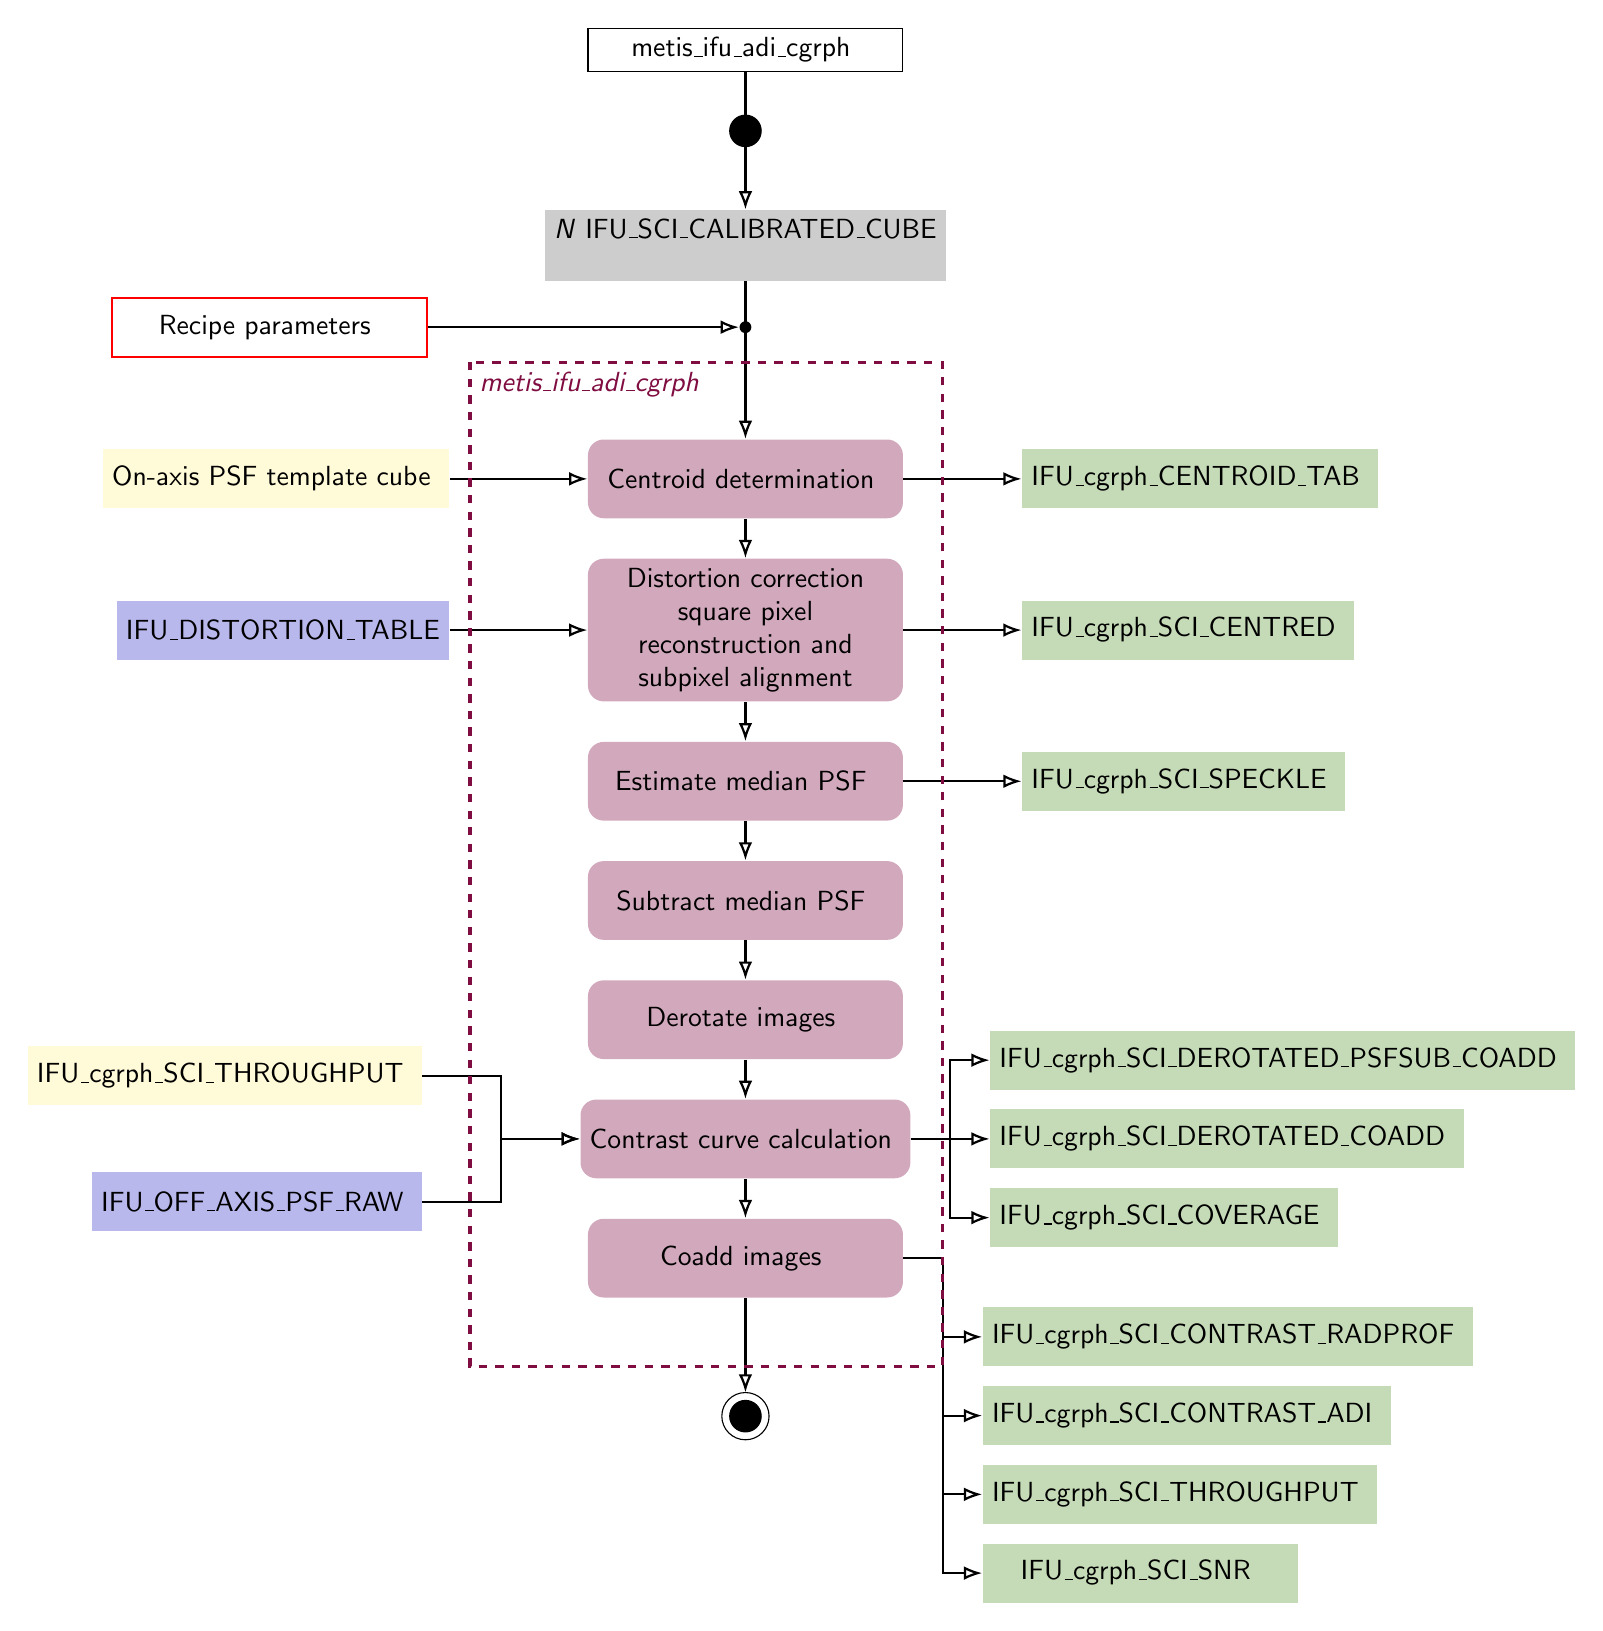
\begin{tikzpicture}
  [x=1cm,
  y=-1cm,
  align=center,
  node distance=2cm and 3cm]
  \sffamily

  %% Grid for orientation. Comment out for final figure!
% \draw[help lines, green](-8, 0) grid (8, 21);

  %%% Put workflow commands here:
  %% Main reduction workflow

  \node (template) [template]{%
   metis\_ifu\_adi\_cgrph
  };

  \pic (start) [below=0.75cm of template] {start};

  \node (input) [below=0.75cm of start-m, input]{%
    \textsl{N} IFU\_SCI\_CALIBRATED\_CUBE\\
    
  };

  \node (step1) [below=2cm of input, redstep]{%
    Centroid determination
  };

  \node (step2)[below=0.5cm of step1, redstep]{%
    Distortion correction\\square pixel\\reconstruction and \\subpixel alignment
  };

  \node (step3) [below=0.5cm of step2, redstep]{%
    Estimate median PSF
  };

  \node (step4) [below=0.5cm of step3, redstep]{%
    Subtract median PSF
  };

  \node (step5) [below=0.5cm of step4, redstep]{%
    Derotate images
  };

  \node (step6) [below=0.5cm of step5, xshift=0cm,redstep]{%
    Contrast curve calculation
  };

  \node (step7) [below=0.5cm of step6, xshift=0cm,redstep]{%
    Coadd images
  };


  \pic (stop) [below=1.5cm of step7]{stop};
  

  %% Connections
  \draw [connection_arrow] (template) -- (input);
  \draw [connection_arrow] (input) -- (step1);
  \draw [connection_arrow] (step1) -- (step2);
  \draw [connection_arrow] (step2) -- (step3);
  \draw [connection_arrow] (step3) -- (step4);
  \draw [connection_arrow] (step4) -- (step5);
  \draw [connection_arrow] (step5) -- (step6);
  \draw [connection_arrow] (step6) -- (step7);
  \draw [connection_arrow] (step7) -- (stop-t);
  

  %% Input
  \node (connectpers) [connection] at
  ($(input)!0.35!(step1)$) {};
  %\node (persistence) [left=3.95cm of connectpers,yshift=0.8cm, external]{%
    %FLUXSTD\_CATALOG
  %};
  %\draw [connection_arrow] (persistence.east) -- ++(1., 0) -- ++(0., 0.8) -- ++(3., 0);

  % Input for detector signature removal (step1)
  %\node (bpmin) [left=2cm of step1, yshift=0.8cm, calproduct]{%
  %  BADPIX\_MAP\_IFU
  %};
  %\draw [connection_arrow] (bpmin.east) -- ++(1., 0) -- ++(0., 0.6) -- ++(1., 0);

  %\node (darkin) [left=2cm of step1, calproduct] {%
  %  MASTER\_DARK\_IFU
  %};
  %\draw [connection_arrow] (darkin) -- (step1);

  %\node (flatin) [left=2cm of step1, yshift=-0.8cm, calproduct]{%
  %  MASTER\_FLAT\_IFU
  %};
  %\draw [connection_arrow] (flatin.east) -- ++(1., 0) -- ++(0., -0.6) -- ++(1., 0);

  % Input for rectification (step3)
  %\node (wavecal) [left=2cm of step3, yshift=0.4cm, calproduct]{%
  %  IFU\_WAVECAL
  %};
  %\draw [connection_arrow] (wavecal.east) -- ++(1., 0) -- %++(0., 0.3) -- ++(1., 0);

  %\node (distortion) [left=2cm of step3, yshift=-0.4cm, calproduct]{%
  %  IFU\_DISTORT\_TAB
  %};
  %\draw [connection_arrow] (distortion.east) -- ++(1., 0) -- ++(0., -0.3) -- ++(1., 0);

  % Further input
  \node (molecparams) [left=3.95cm of connectpers,yshift=0cm, params]{%
    Recipe parameters
  };
  \draw [connection_arrow] (molecparams.east) -- (connectpers);%-- ++(0.25, 0) -- ++(0., -0.8) -- ++(3.75, 0);

  %\node (stdcat) [left=2cm of step5, external] {%
   % FLUXSTD\_CATALOG
  %};
  %\draw [connection_arrow] (stdcat.east) -- (step5);

  %% Output
  %\node (connectreduced) [connection] at
 % ($(step5)!0.4!(stop-t)$) {};

\node (incont1) [left=2cm of step6, yshift=0.8cm,calib]{%
    IFU\_cgrph\_SCI\_THROUGHPUT
  };
\draw [connection_arrow] (incont1.east) -- ++(1, 0) -- ++(0., 0.8) -- ++(1, 0);

\node (incont2) [left=2cm of step6, yshift=-0.8cm,calproduct]{%
    IFU\_OFF\_AXIS\_PSF\_RAW
  };
\draw [connection_arrow] (incont2.east) -- ++(1, 0) -- ++(0., -0.8) -- ++(1, 0);

\node (outcont1) [right=1.cm of step6, yshift=1cm,sciproduct]{%
    IFU\_cgrph\_SCI\_DEROTATED\_PSFSUB\_COADD
  };
\draw [connection_arrow] (step6.east) -- ++(0.5, 0) -- ++(0., -1) -- ++(0.5, 0);

\node (outcont2) [right=1.cm of step6, yshift=0cm,sciproduct]{%
    IFU\_cgrph\_SCI\_DEROTATED\_COADD
  };
\draw [connection_arrow] (step6.east) -- (outcont2);

\node (outcont3) [right=1.cm of step6, yshift=-1cm,sciproduct]{%
    IFU\_cgrph\_SCI\_COVERAGE
  };
\draw [connection_arrow] (step6.east) -- ++(0.5, 0) -- ++(0., 1) -- ++(0.5, 0);

\node (outcont4) [right=1.cm of step7, yshift=-1cm,sciproduct]{%
    IFU\_cgrph\_SCI\_CONTRAST\_RADPROF
  };
\draw [connection_arrow] (step7.east) -- ++(0.5, 0) -- ++(0., 1) -- ++(0.5, 0);

\node (outcont5) [right=1.cm of step7, yshift=-2cm,sciproduct]{%
    IFU\_cgrph\_SCI\_CONTRAST\_ADI
  };
\draw [connection_arrow] (step7.east) -- ++(0.5, 0) -- ++(0., 2) -- ++(0.5, 0);

\node (outcont6) [right=1.cm of step7, yshift=-3cm,sciproduct]{%
    IFU\_cgrph\_SCI\_THROUGHPUT
  };
\draw [connection_arrow] (step7.east) -- ++(0.5, 0) -- ++(0., 3) -- ++(0.5, 0);

\node (outcont7) [right=1.cm of step7, yshift=-4cm,sciproduct]{%
    IFU\_cgrph\_SCI\_SNR
  };
\draw [connection_arrow] (step7.east) -- ++(0.5, 0) -- ++(0., 4) -- ++(0.5, 0);

\node (reduced2) [right=1.5cm of step1, sciproduct]{%
    IFU\_cgrph\_CENTROID\_TAB
  };
  \draw [connection_arrow] (step1) -- (reduced2);
 
  \node (reduced) [right=1.5cm of step2, sciproduct]{%
    IFU\_cgrph\_SCI\_CENTRED
  };
  \draw [connection_arrow] (step2) -- (reduced);

  \node (reduced3) [left=1.75cm of step2, calproduct]{%
    IFU\_DISTORTION\_TABLE};
  \draw [connection_arrow] (reduced3) -- (step2);
 
  \node (reduced4) [left=1.75cm of step1, calib]{%
    On-axis PSF template cube
  };
  \draw [connection_arrow] (reduced4) -- (step1);
 % \node (connectfluxcal) [connection] at
 % ($(step5)!0.8!(stop-t)$) {};
  \node (fluxcal) [right=1.5cm of step3, sciproduct]{%
    IFU\_cgrph\_SCI\_SPECKLE
  };
  \draw [connection_arrow] (step3) -- (fluxcal);

  %% Frame around recipe
  \draw [frame] ($(input)!0.5!(step1) - (3.5,0)$)
  rectangle ($(step7)!0.75!(stop-t) + (2.5,0)$);
  \node [framecolor, anchor=north west] at
  ($(input)!0.5!(step1) - (3.5, 0)$) {%
    \textsl{metis\_ifu\_adi\_cgrph}};

\end{tikzpicture}

% ADDING NEW DEFINITIONS -------------------------------------------- start
\definecolor{listingbg}{gray}{0.95}
\definecolor{darkgreen}{rgb}{0.0, 0.7, 0.0}
\definecolor{darkblue} {rgb}{0.0, 0.0, 0.7}
\definecolor{cyan} {rgb}{0.0, 0.4, 0.4}
\definecolor{darkred}  {rgb}{0.7, 0.0, 0.0}
\definecolor{darkorange}{rgb}{1.0, 0.49, 0.0}
\definecolor{violet}{rgb}{255, 0, 255}
\definecolor{turq}{rgb}{0.0, 0.7, 0.8}
\definecolor{fits}{rgb}{0.4, 0.1, 1}


\makeatletter
\lstdefinestyle{RAWstyle}{%
  basicstyle=\ttfamily\color{fits}%
  \lst@ifdisplaystyle\scriptsize\fi}

\lstdefinestyle{PARstyle}{%
  basicstyle=\ttfamily\color{cyan}%
  \lst@ifdisplaystyle\scriptsize\fi}

\lstdefinestyle{DRLstyle}{%
  basicstyle=\ttfamily\color{violet}%
  \lst@ifdisplaystyle\scriptsize\fi}

\lstdefinestyle{RECstyle}{%
  basicstyle=\ttfamily\color{darkgreen}%
  \lst@ifdisplaystyle\scriptsize\fi}

%% Write QC parameters like this: \QC{QC_SOMETHING_OR_OTHER}
\lstdefinestyle{QCstyle}{%
  basicstyle=\ttfamily\color{darkblue}%
  \lst@ifdisplaystyle\scriptsize\fi}

%% Write templates like this: \TPL{DARK_LM}
\lstdefinestyle{TPLstyle}{%
  basicstyle=\ttfamily\color{darkred}%
  \lst@ifdisplaystyle\scriptsize\fi}

%% Write products like this: \hyperref[dataitem:some_thing]{\PROD{SOME_THING}}
\lstdefinestyle{PRODstyle}{%
  basicstyle=\ttfamily\color{darkorange}%
  \lst@ifdisplaystyle\scriptsize\fi}

%% external calib files
\lstdefinestyle{EXTCALIBstyle}{%
  basicstyle=\ttfamily\color{Turquoise}%
  \lst@ifdisplaystyle\scriptsize\fi}

% static calib files
\lstdefinestyle{STATCALIBstyle}{%
  basicstyle=\ttfamily\color{teal}%
  \lst@ifdisplaystyle\scriptsize\fi}
\makeatother



  \caption[Recipe: \REC*{metis_ifu_adi_cgrph}]{\REC*{metis_ifu_adi_cgrph} -- IFU ADI post processing for RAVC/CVC coronagraph.
    }
  \label{fig:metis_ifu_adi_cgrph}
\end{figure}
\restoregeometry

%%% Local Variables:
%%% TeX-master: "METIS_DRLD"
%%% End:
